% Chapter Template

\chapter{Background} % Main chapter title

\label{Background} % Change X to a consecutive number; for referencing this chapter elsewhere, use \ref{ChapterX}

%----------------------------------------------------------------------------------------
%	ASR
%----------------------------------------------------------------------------------------

\section{Automatic Speech Recognition}

Automatic speech recognition models can be split into two general categories of complexity. First of all, there is single-word classification to an isolated vocabulary where directed dialogue conversations (DDC) are analyzed; its overall capabilities can be seen in early ASR efforts such as IBM’s Shoebox. The other variant is continuous speech recognition, where natural language conversations (NLCs) are processed and transcribed to a vocabulary of around 20,000 to 100,000 words. Many technologies today utilize this system, including video subtitles, voice input systems, and customer services at call centres. While DDC classification models can be fairly simple to understand and produced through feed-forward networks, continuous NLC networks require the use of recurrent neural networks.

%-----------------------------------
%	RNN
%-----------------------------------
\section{Recurrent Neural Networks for ASR}

Recurrent neural networks (RNNs) are a variant of deep learning neural networks that use time-sequential data without a fixed input shape. These systems are inspired by the biological composition of neurons in the brain; modern society often adapts its greatest innovations from nature. Each neuron, out of around 100 million, is interconnected with one another and passes a signal via its axon to receiving axon terminals belonging to other neurons~\cite{koehn_2020}. Similarly, in an artificial linear neural network, a combination of weights and biases stacked in layers are constantly optimized through gradient descent to produce a matrix of probabilities that highlight the best possible output the network can generate in its current state. In each cell, a dot product of the input matrix and the cell’s weight matrix is done and summed with the cell’s bias matrix to create an output matrix of values, which is eventually fed into a proceeding layer of nodes (Figure~\ref{fig:FeedForwardNN})~\cite{koehn_2020}.

\begin{figure}[th]
    \centering
    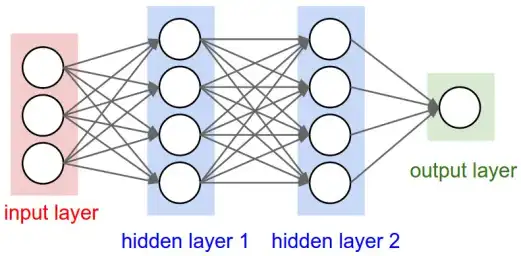
\includegraphics[width=0.5\textwidth]{Figures/neuralnet.png}
    \[ y = w\cdot{x} + b \]
    w: weights, b: biases
    \decoRule
    \caption[Feed Forward Neural Network]{The nodal, layer-by-layer architecture of a feed-forward neural network (Source: Mukul Rathi)}
    \label{fig:FeedForwardNN}
\end{figure}

At first, these matrices carry out operations using senseless, randomly generated weights and biases that result in a completely random output. However, as the model calculates its loss from an evaluation of the net deviation of the predicted output from the ground truth, a gradient is formulated that adjusts each layer’s parameters closer to what would create an output with a lower loss~\cite{koehn_2020}. The higher loss an output receives, the greater magnitude of the gradient is passed to backpropagation and the more each node in the network is changed, with the vice versa applying as well.
\par
In a typical feed-forward neural network, the input and output shapes of the model are fixed and have to be consistent in order to be trained properly. Since the length of the NLC audio input can vary in this investigation, recurrent neural networks will be used to process continuous speech data that last an indeterminate length of time. RNNs accomplish this task by accepting input for each time step into a recurrent cell and feeding the cell’s generated output to the succeeding cell through a hidden layer that stores a certain number of hidden units, doing so until it reaches the end of the input batch~\cite{graves_mohamed_hinton_2013,koehn_2020}. This results in the interconnected nature of a recurrent neural network that enables it to find relationships in continuous data~\cite{ibm_cloud_education_2020}, namely in stock market prediction, and influence future outputs. The framework of a standard RNN cell is laid out below (Figure~\ref{fig:RNNCell}), where xt is the inputted time step data, ot is the cell output after the tanh function is carried out, ht-1 is the previous cell’s hidden output, and ht is the current cell’s hidden output to be sent to the next cell.

\begin{figure}[th]
    \centering
    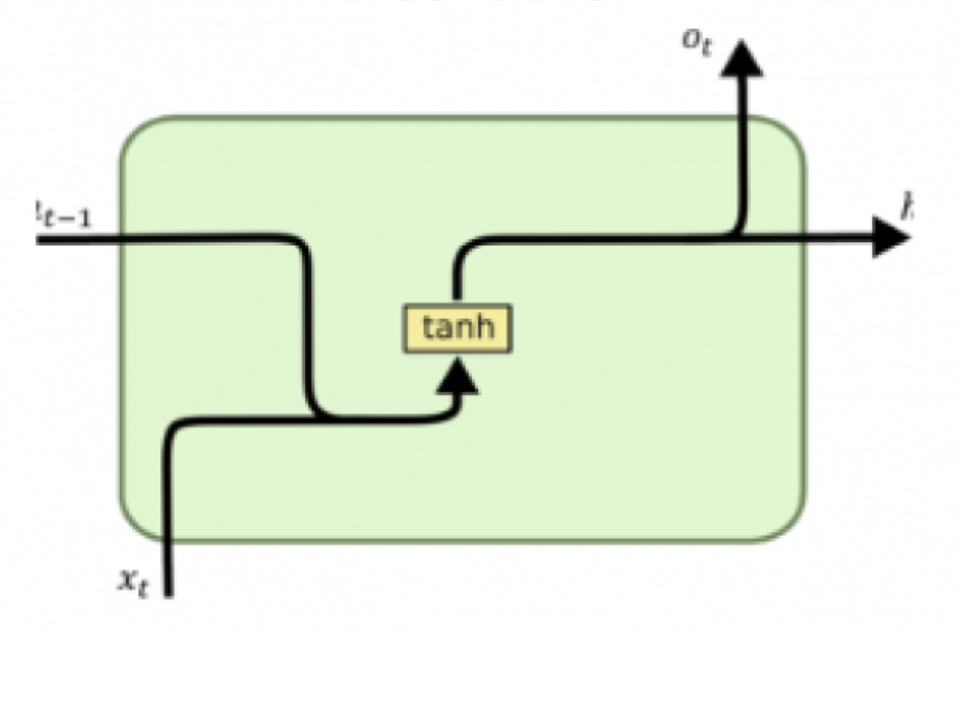
\includegraphics[width=0.5\textwidth]{Figures/rnnarch.png}
    \[ h_t = \tanh(W(
        \begin{pmatrix}
            h_{t-1} \\ x_t
        \end{pmatrix}
    )) \]
    \decoRule
    \caption[RNN Cell]{The internal composition of a recurrent network cell (Source: Lopez~\cite{lopez_2019})}
    \label{fig:RNNCell}
\end{figure}

The distribution of input data and output data can vary from network to network and is ultimately based on the shape of the input data and the desired shape of the output data, unlike feedforward networks~\cite{ibm_cloud_education_2020}. For example, a music generation RNN could take in a dataset of Vivaldi’s works as an input and output an infinite length of completely original Vivaldi-styled music: this model would be classified as a one-to-many RNN structure. Table~\ref{tab:RNNStructures} describes four main types of RNN structures that satisfy most criteria of networks that use continuous data.

\begin{table}
    \centering
    \begin{tabular}{p{0.16\textwidth}p{0.23\textwidth}p{0.24\textwidth}p{0.15\textwidth}}
        \toprule
        \textbf{Architecture} & \textbf{Characteristics} & \textbf{Application} & \textbf{Diagram} \\
        \midrule

        One-to-One & Single input \newline Single output & Image classification & 
        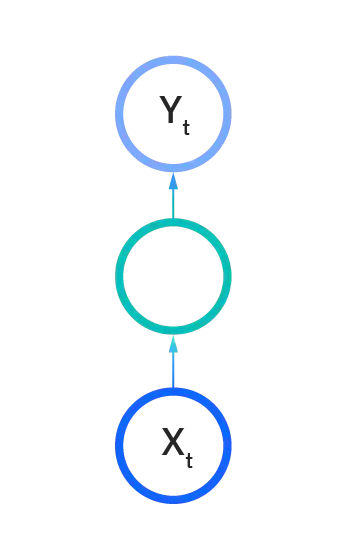
\includegraphics[width=0.08\textwidth]{Figures/onetoone.png} \\

        One-to-Many & Single input \newline Sequence of outputs & Image captioning & 
        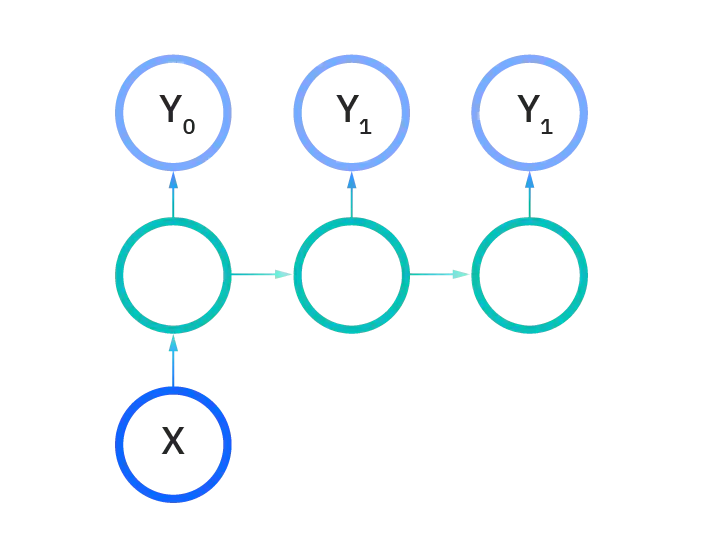
\includegraphics[width=0.16\textwidth]{Figures/onetomany.png} \\

        Many-to-One & Sequence of inputs \newline Single output & Sentiment analysis & 
        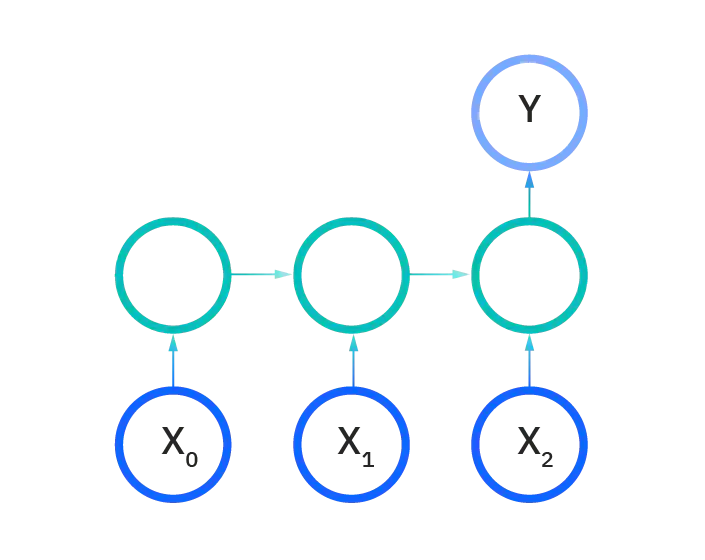
\includegraphics[width=0.16\textwidth]{Figures/manytoone.png} \\

        Many-to-Many & Sequence of inputs \newline Sequence of outputs & Language translation & 
        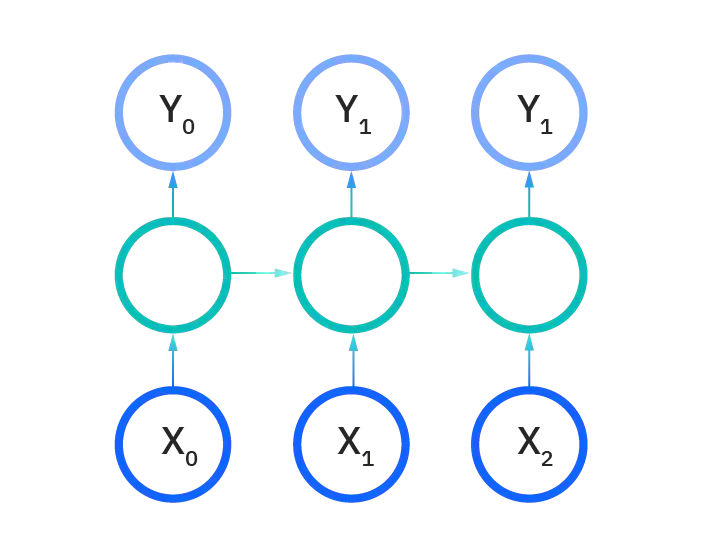
\includegraphics[width=0.16\textwidth]{Figures/manytomany.png} \\

        \bottomrule\\
    \end{tabular}
    \caption{Four types of recurrent neural network structures (Source: IBM~\cite{ibm_cloud_education_2020})}
    \label{tab:RNNStructures}
\end{table}

Due to the continuous nature of transcribing NLCs, there are an indeterminate number of inputs and outputs present.  Thus, a many-to-many RNN structure will be used as the framework for this investigation’s experimentation. Additionally, many high-performance NLC RNNs include another layer of recurrent cells that examines the input data in reverse as well, called bidirectional RNNs, in order to better distinguish the meaningful attributes and relationships in language.
\par
However, conventional recurrent neural networks have two major problems that need to be considered: the vanishing and exploding gradient problem, and a long-term dependency on speech waveforms. The vanishing and exploding gradient problem appear during the backpropagation stage of the network, where a gradient propagates through each cell and updates the weights and biases of each node for the network to learn~\cite{mehrotra_2021}. The problem arises when the number of layers starts to increase and the gradients start to travel and multiply through more and more layers; when a gradient with a slight deviation from 1 is returned to the first node during backpropagation, it begins to increase or decrease exponentially as it progresses through each cell. Correspondingly, as it reaches the end of backpropagation, the gradient is either too minuscule to the point where the end weight is scarcely updated at all, or too large where the weight cannot be adequately optimized~\cite{brownlee_2021,mehrotra_2021}.
\par
Going on, audio waveforms can take up a significant portion of input data, dependent on sample frequency, as a one-second audio clip of someone dictating a word can take up to 16,000 time steps of data at a sample rate of 16 kHz. The extreme short-term memory of a simple hyperbolic tangent recurrent network cannot remember what sound signal was inputted into the cell 5,000 iterations earlier, to the extent that it is significant towards producing the output. This is detrimental towards the ultimate performance of the neural network, as a large segment of a model’s decision on a phoneme, character, or word depends on contextual data beforehand~\cite{koehn_2020}. For example, a model could have difficulties discriminating between the letter “k” and “q” with no context. However, the prerequisite knowledge that it was preceded by a “loo” will likely increase the probability that the following letter is “k”. These two setbacks of recurrent neural networks introduced a revolutionary recurrent cell concept first established in 1997 and prominently used today, termed the Long Short-Term Memory cell~\cite{brownlee_2021}.


%-----------------------------------
%	LSTM
%-----------------------------------
\section{Long Short-Term Memory}

Long Short-Term Memory (LSTM) cells counter the two problems above by incorporating an extra hidden memory state that propagates throughout recurrences of the network. Adding a memory state that can remember important specifics from many recurrences beforehand influences the current output~\cite{brownlee_2021,koehn_2020}. Contrary to the perception-based framework of traditional neural networks, an LSTM cell is much more convoluted and contains substantially more weights and biases in the form of specialized gates: the forget gate, input gate, and output gate (Figure~\ref{fig:LSTMCell}), each with a specialized purpose~\cite{koehn_2020,lendave_2021}. The combination of these properties provides the fundamental framework that conceives the LSTM network’s ability to recognize context-sensitive information and is the reason why these networks are the standard for building reliable speech recognition systems. 

\begin{figure}[th]
    \centering
    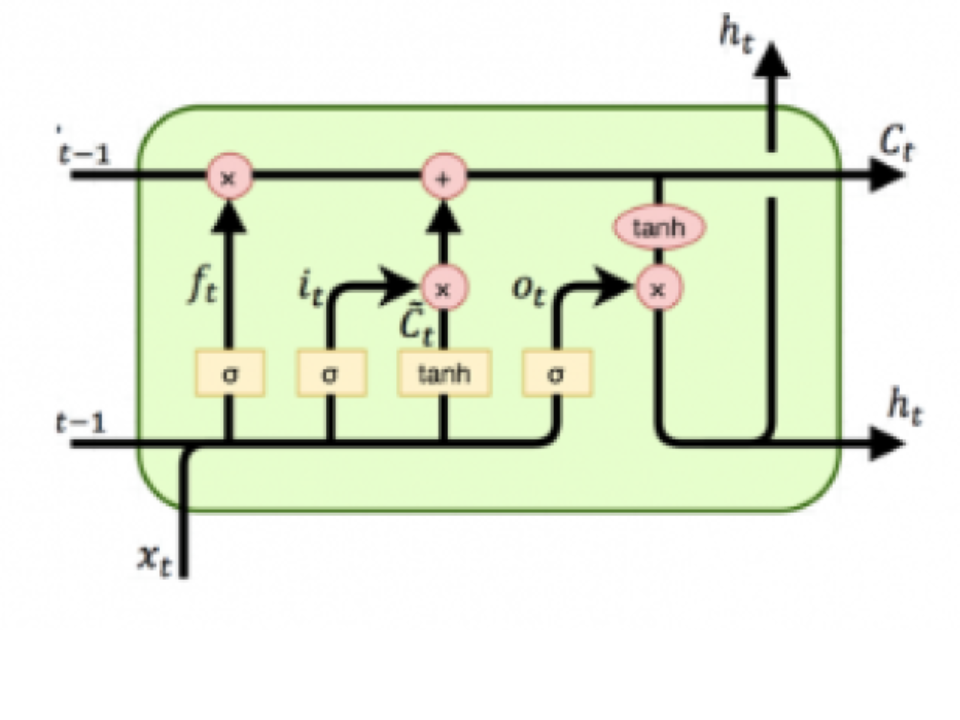
\includegraphics[width=0.5\textwidth]{Figures/lstmarch.png}
    \begin{gather*}
    \begin{pmatrix}
        i_{gate} \\ f_{gate} \\ o_{gate} \\ g_{gate}
    \end{pmatrix}
    =
    \begin{pmatrix}
        \sigma \\ \sigma \\ \sigma \\ \tanh
    \end{pmatrix}
    W
    \begin{pmatrix}
        h_{t-1} \\ x_t
    \end{pmatrix}\\
    c_t = f \cdot c_{t-1} + i \cdot g\\
    h_t = o \cdot \tanh(c_t)
    \end{gather*}
    \decoRule
    \caption[LSTM Cell]{The internal composition of an LSTM cell (Source: Lopez~\cite{lopez_2019})}
    \label{fig:LSTMCell}
\end{figure}

A simple speech recognition system is usually composed of two different components: a feature extraction layer and the neural network itself. The purpose of the feature extraction layer is to process the raw input data into a more usable form that captures a certain aspect of sound~\cite{janse_magre_kurzekar_deshmukh_2014}. In the case of ASR, input data is typically in the form of waveform data embedded in mp3 or wav files. This one-dimensional waveform data has several limitations due to having less useful features and larger variability in the speech signal than a two-dimensional format of audio signals~\cite{janse_magre_kurzekar_deshmukh_2014}, such as spectrograms. Spectrograms are a visual representation of the amplitudinal spectrum of frequencies of an audio signal with respect to time\cite{mahanta_padmanabhan_2021}. These amplitude maps of frequency can be extracted through the discrete short-time Fourier transform (STFT), which splits an audio sample into smaller segments of waveform data and processes the segment through a Fourier transform to represent the waveform as a set of frequencies for a frame of time~\cite{smith_2007}. Concatenating these frames together creates a two-dimensional time series of frequencies that are called spectrograms. The discrete STFT function is defined as:

\begin{align*}
    X\left[n,w\right[ = \sum_{m=-\infty}^{\infty}w[n-m]\cdot~x[m]\cdot~e^{-iwm}\\
    n: frame index, w: frequency
\end{align*}

Spectrograms are frequently used in convolutional neural networks due to their multi-dimensional property and are the reliable standard in terms of extracting audio features from waveform data since they can accurately represent their original audio signals~\cite{green_2018}. In a spectrogram, the x-axis refers to time and the y-axis refers to the frequency that’s played at a certain point in time, with a lighter colour indicating that the amplitude is larger with regard to magnitude (Figure~\ref{fig:Spectrogram})~\cite{green_2018}.

\begin{figure}[th]
    \centering
    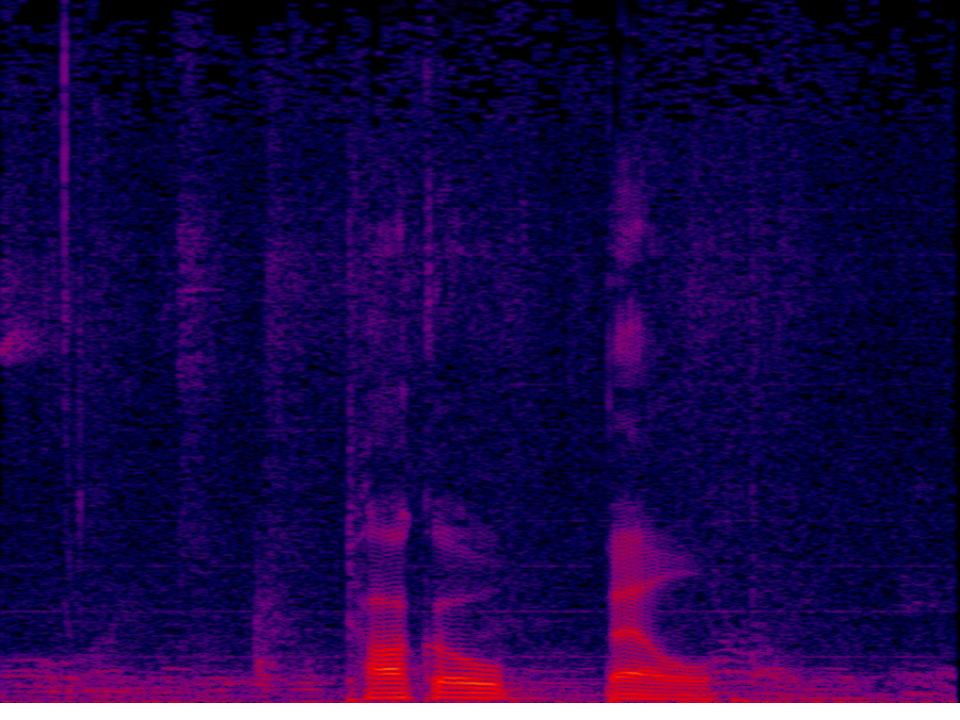
\includegraphics[width=0.5\textwidth]{Figures/tacobell.png}
    \decoRule
    \caption[Spectrogram]{A spectrogram of a person saying the phrase, "Taco Bell"}
    \label{fig:Spectrogram}
\end{figure}

%-----------------------------------
%	Feature Extraction Algorithms
%-----------------------------------
\section{Feature Extraction Algorithms}

However, spectrograms are not very well suited nor optimized for visualizing human speech. For instance, a human voice at a conversational level will normally not exceed a frequency range between 60 Hz and 500 Hz and it’s not necessary to include non-phonetically vital properties of speech signals in the input data. Therefore, Mel-frequency spectrograms were intended to artificially replicate the human hearing system on how we perceive different frequencies [21, towardsdatascience]. Mel spectrograms are computed through a precise logarithm function, dubbed the Mel-frequency filter bank, which retains the phonetically vital properties of speech signals and plots the result on the Mel scale (Figure~\ref{fig:Melscale})~\cite{li_2015}.

\begin{figure}[th]
    \centering
    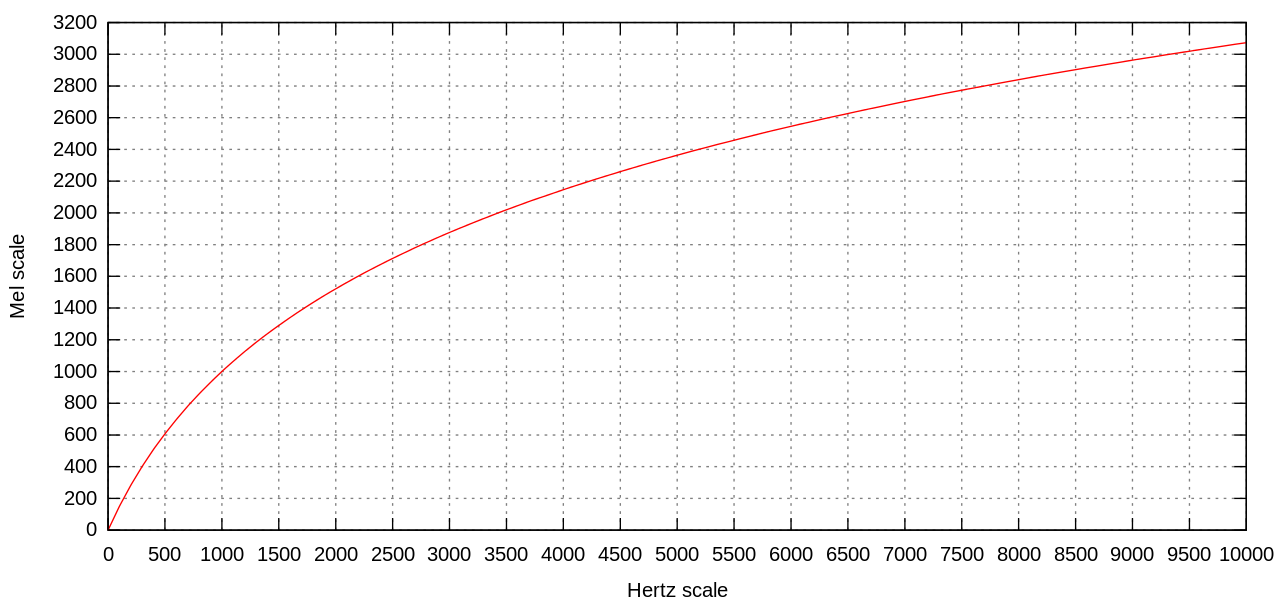
\includegraphics[width=0.7\textwidth]{Figures/melscale.png}
    \[mel(f) = 2595 x \log_10(1+ f/700)\]
    \decoRule
    \caption[Melscale]{The logarithmic relationship between the Hertz and Mel scale (Source: Vedala~\cite{vedala_2022})}
    \label{fig:Melscale}
\end{figure}

On the other hand, Mel-Frequency Cepstrum Coefficients are a set of coefficients that represent the changes in a spectrum of Mel frequencies over time~\cite{janse_magre_kurzekar_deshmukh_2014}. The process involved in developing MFCCs includes taking the logarithm of a Mel spectrogram and applying the inverse discrete cosine transform to create a cepstrum of the original spectrum~\cite{singh_2019}. The result is a small set of coefficients, typically around 10-20, that ultimately represent the main speech features of the original waveform data. The number of coefficients outputted can be tuned as a hyperparameter to represent different types of audio data optimally. The small space complexity of MFCCs results in fast training and prediction times.
\par
Another speech feature extraction function that will be evaluated is discrete wavelet transforms (DWTs). DWTs decompose a signal using a defined set of wavelets at a particular set of scales to represent the waveform and can extract local spectral and temporal information simultaneously~\cite{nechyba_2004,talebi_2022}. It uses an algorithm similar to the STFT in addition to convolutions in convolutional neural networks. A specific wavelet, or window, “slides” through the input and multiplies itself with the input waveform~\cite{talebi_2022,nehe_holambe_2012}, creating a convolutional output. The wavelet executes multiple passes through the waveform, changing its wavelength each time, and outputs how much of the wavelet is within a signal, similar to how kernels behave in convolutional neural networks~\cite{nehe_holambe_2012} (Figure~\ref{fig:DWT}).

\begin{figure}[th]
    \centering
    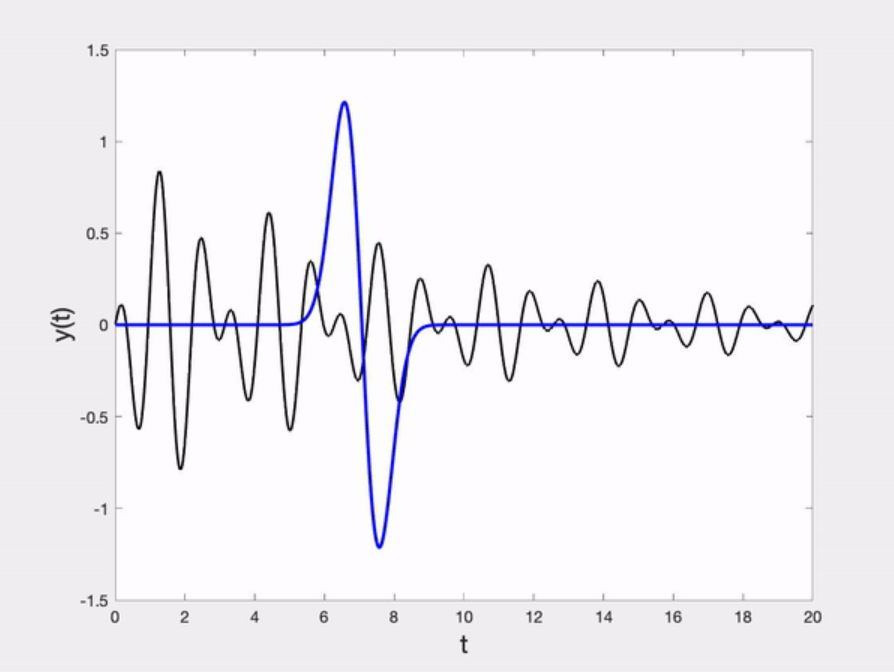
\includegraphics[width=0.5\textwidth]{Figures/dwt.png}
    \decoRule
    \caption[DWT]{A wavelet traversing through a waveform (Source: Towards Data Science~\cite{talebi_2022})}
    \label{fig:DWT}
\end{figure}

The DWT of a signal is determined/specified by the function~\cite{nehe_holambe_2012}:
\begin{gather*}
    T_{m,n}=\int_{-\infty}^{\infty}x(t)\cdot~\psi({t-n}/m) dt\\
    \psi: wavelet, m: scaling factor, n: translation parameter
\end{gather*}